% !TEX root = ../acsfubAuthorGuidelines-short.tex
\documentclass{standalone}
\usepackage{tikz}
\usetikzlibrary{positioning,calc}
\usepackage{csquotes}
\usepackage{hyperref}
\usepackage{subfigure}
\usepackage{pgfplotstable}
\pgfplotsset{compat=1.18}

\usepackage{xcolor}
\definecolor{myLightGray}{HTML}{F1F1F1}

\begin{document}
\color{myLightGray}
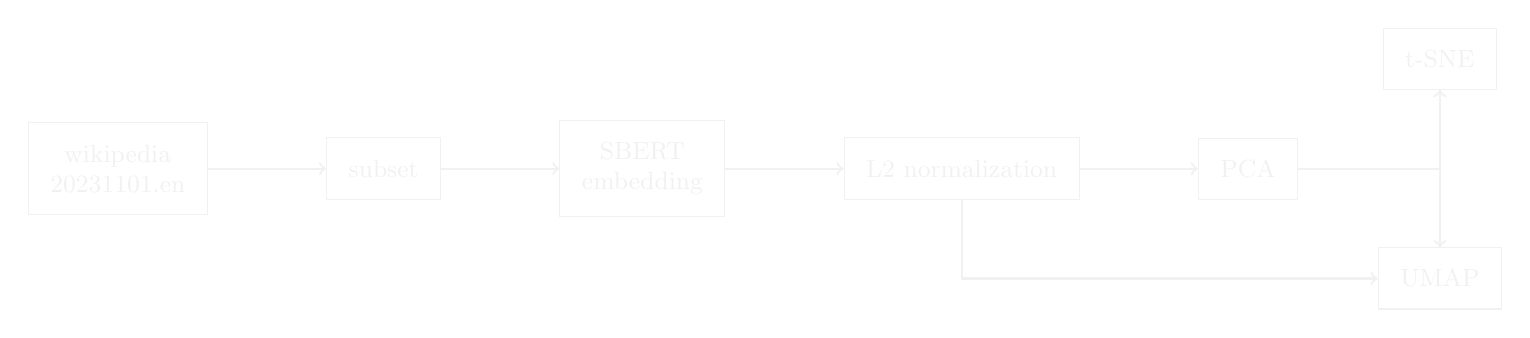
\begin{tikzpicture}[
        scale=0.9,
        node distance=1cm and 1.5cm,
        box/.style={draw=myLightGray, rectangle, align=center, font=\small, inner sep=0.28cm, text=myLightGray}, % Apply color to draw and text
        arrow style/.style={->, myLightGray, thick} % Define a style for arrows
    ]
    \node[box] (A) {wikipedia\\20231101.en};
    \node[box, right=of A] (B) {subset};
    \node[box, right=of B] (C) {SBERT\\embedding};
    \node[box, right=of C] (D) {L2 normalization};
    \node[box, right=of D] (F) {PCA};

    \coordinate (split) at ($(F.east)+(2,0)$);

    \node[box, above=of split] (G) {t-SNE};
    \node[box, below=of split] (H) {UMAP};

    \draw[arrow style] (A) -- (B); % Use the arrow style
    \draw[arrow style] (B) -- (C);
    \draw[arrow style] (C) -- (D);
    \draw[arrow style] (D) -- (F);
    \draw[arrow style] (D) |- (H);

    \draw[arrow style] (F.east) -- (split) -| (G.south);
    \draw[arrow style] (F.east) -- (split) -| (H.north);
\end{tikzpicture}
\end{document}